\documentclass[12pt]{report}

% Languages and fonts
\usepackage{polyglossia}
\setdefaultlanguage{greek}
\setotherlanguage{english}
\usepackage{fontspec}
\renewcommand{\thesection}{\arabic{section}} % Begin sections from 1
\setmainfont{Times New Roman} % Set main font to Times New Roman

% Images
\usepackage{graphicx}
\usepackage{float} % placement of figures

% Math
\usepackage{amsmath} % mathematica symbols 
\usepackage{mathrsfs} % curly math letters
\usepackage{amssymb} %more mathematical symbols
\usepackage{gensymb} % degree symbol
\usepackage{mathtools} % For \mathclap

% Miscellaneous
\usepackage{parskip} % Remove paragraph indentation
\usepackage{enumitem} % For custom itemizes
\usepackage{hyperref} % For hyperlinks and references
% \usepackage{booktabs}

\begin{document}

\begin{titlepage}
\begin{center}
    \begin{figure}[h]
        \centering
        
\includegraphics[width=1\textwidth]{figures/auth_logo.png}
    \end{figure}

    \vspace{1cm}

    \Huge
    \textbf{1η Εργασία}

    \vspace{2cm}
    
    Υπολογιστική Νοημοσύνη \\

    \vspace{2cm}

    \Large
    Παπαδάκης Κωνσταντίνος Φώτιος \\
    ΑΕΜ: 10371

    \vfill

    \large
    Αριστοτέλειο Πανεπιστήμιο Θεσσαλονίκης \\
    Τμήμα Ηλεκτρολόγων Μηχανικών και Μηχανικών Υπολογιστών \\
    \today
\end{center}
\end{titlepage}

\tableofcontents

\newpage

\section{Περιγραφή Συστήματος}
Επιλέγοντας ελεγκτή PI έχουμε:
\begin{equation}
    \label{eq:pi_controller}
    G_c(s) = K_P + \frac{K_I}{s} = \frac{K_P \cdot s +K_I}{s} = \frac{K_P(s+\frac{K_I}{K_P})}{s} = \frac{K(s+c)}{s}
\end{equation}

Γνωρίζοντας ότι το σύστημα με τον κινητήρα μας είναι:
\begin{equation}
    \label{eq:closed_loop_system}
    H(s) = \frac{25}{(s+0.1)(s+10)}
\end{equation}

Η συνάρτηση μεταφοράς ανοικτού βρόγχου προκύπτει ως εξής:
\begin{equation}
    \label{eq:open_loop_transfer_function}
    H(s)G_c(s) = A(s) = \frac{K(s+c)}{s(s+0.1)(s+10)}
\end{equation}

Καθώς έχουμε μοναδιαία αρνητική ανάδραση η συνάρτηση κλειστού βρόγχου μπορεί να υπολογιστεί από τη σχέση:
\begin{equation}
    \label{eq:closed_loop_transfer_function}
    H_c(s) = \frac{A(s)}{1+A(s)} = \frac{K(s+c)}{s(s+0.1)(s+10) + K(s+c)}
\end{equation}

Η βηματική ανάδραση του συστήματος κλειστού βρόγχου είναι:
\begin{equation}
    \label{eq:closed_loop_step_response}
    Y(s) = H_c(s) \cdot X(s) = \frac{H_c(s)}{s} = \frac{K(s+c)}{s[s(s+0.1)(s+10) + K(s+c)]}
\end{equation}

\section{Επιλογή Ελεγκτή}
Έχω δύο προδιαγραφές που πρέπει να ικανοποιούνται προκειμένου να επιλέξω τον σωστό ελεγκτή:
\begin{enumerate}[label=(\alph*)]
    \item Υπερύψωση για βηματική είσοδο  $<8\%$.
    \item Χρόνος ανόδου $<0.6s$.
\end{enumerate}

Μέσω της συνάρτησης \textbf{checkViability()} περνώ ως παράμετρο την συνάρτηση μεταφοράς κλειστού βρόγχου (Σχέση \ref{eq:closed_loop_system}) και αυτή ελέγχει τις παραπάνω συνθήκες. Η συνάρτηση \textbf{createViableckCSV()} από την άλλη, αξιοποιεί την \textbf{checkViability()} ανατρέχοντας στις διάφορες πιθανές τιμές που μπορούν να πάρουν τα K (φυσικοί αριθμοί από το 1 μέχρι το 100) και c (δεκαδικοί αριθμοί ενός ψηφίου υποδιαστολής από το -0.1 μέχρι το -10). Εν τέλει παράγει ένα αρχείο CSV με ικανά ζεύγη τιμών, από το οποίο επιλέγουμε αυθαίρετα το ζεύγος $(K, c)=(0.3, 30)$.

Έτσι έχουμε:
\begin{align*}
    K = K_P &= 30 \\
    c = \frac{K_I}{K_P} &= 0.3 \Rightarrow K_I = 9\\
\end{align*}

\section{Γεωμετρικός Τόπος Ριζών}
\subsection{Απεικόνιση Matlab}
Ο ΓΤΡ (Γεωμετρικός Τόπος Ριζών) της συνάρτησης μεταφοράς ανοικτού βρόγχου (Σχήμα \ref{fig:root_locus}) έχει δύο ασύμπτωτες ευθείες $90\degree$ και $-90\degree$ μοιρών.
\begin{figure}[H]
    \centering
    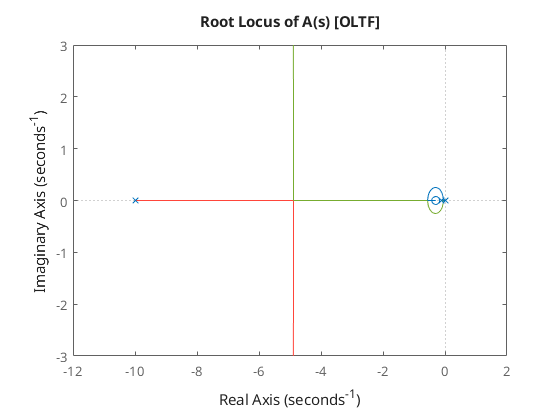
\includegraphics[width=0.8\textwidth]{figures/root_locus.png}
    \caption{Γεωμετρικός Τόπος Ριζών Συστήματος}
    \label{fig:root_locus}
\end{figure}

\subsection{Θεωρητική Ανάλυση}
Πόλοι:  
\begin{align*}
    s(s+0.1)(s+10) &= 0 \\
    s_1 &= 0 \\
    s_2 &= -0.1 \\
    s_3 &= -10 \\
\end{align*}

Μηδενικά:
\begin{align*}
    K(s+c) &= 0 \\
    s &= -c = -0.3 \\
\end{align*}

Συνεπώς:
\begin{align*}
    \left.
    \begin{aligned}
        n &= \text{αριθμός πόλων} = 3 \\
        m &= \text{αριθμός μηδενικών} = 1 
    \end{aligned}
    \quad
    \right\}
    \Rightarrow 
    \quad
    n-m = 2
\end{align*}

Ασύμπτωτες:
\begin{align*} % * is used to omit numbering
    \theta_i &= \frac{(2i+1)180\degree}{n-m} \\
    \theta_0 &= \frac{(2 \cdot 0+1)180\degree}{2} = \frac{180\degree}{2} = 90\degree \\
    \theta_1 &= \frac{(2 \cdot 1+1)180\degree}{2} = \frac{(3)180\degree}{2} = 270\degree \equiv -90\degree\\
\end{align*}

Σημείο τομής ασύμπτωτων με τον πραγματικό άξονα:
\begin{align*}
    \sigma_A &= \frac{\sum_{i=1}^{n} p_i - \sum_{i=1}^{m} z_i}{n-m} \\
    \sigma_A &= \frac{0 + (-0.1) + (-10) - (-0.3)}{2} \\
    \sigma_A &= \frac{-9.8}{2} \\
    \sigma_A &= -4.9
\end{align*}

Σημεία Σύγκλισης και Απόσχισης:
\begin{align*}
    H_p(s) &= \frac{s+0.3}{s(s+0.1)(s+10)} \\
    \frac{dH_p(s)}{ds} &= 0 \\
    0 &= \frac{s(s+0.1)(s+10) - (s+0.3)(3s^2+20s+0.2s+1)}{[s(s+0.1)(s+10)]^2} \\
    0 &= s(s+0.1)(s+10) - (s+0.3)(3s^2+20.2s+1) \\
    0 &= -2s^3 -11s^2 -6.06s -0.3 \\
    s_1 &= -4.88616 \\
    s_2 &= -0.0549265 \\
    s_3 &= -0.558009
\end{align*}
Έτσι:
\begin{itemize}
    \item Το σημείο $s_1$ είναι το σημείο από το οποίο οι πόλοι -0.1 και -10 αναχωρούν προς τις δύο ασύμπτωτες.
    \begin{figure}[H]
        \centering
        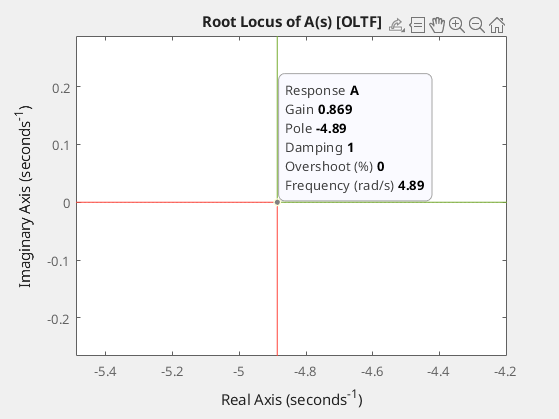
\includegraphics[width=0.8\textwidth]{figures/root_locus_s1.png}
        \caption{Σημείο Απόσχισης $s_1$}
        \label{fig:root_locus_s1}
    \end{figure}
    \item Το σημείο $s_2$ είναι το σημείο απόσχισης των πόλων 0 και -0.1. Διαγράφουν ελειψοειδή πορεία και συγκλίνουν στο σημείο $s_3$.
    \begin{figure}[H]
        \centering
        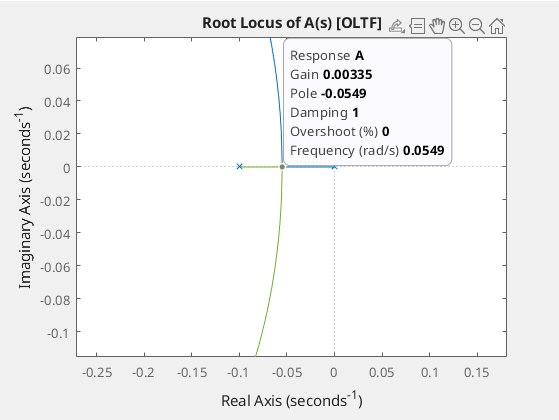
\includegraphics[width=0.8\textwidth]{figures/root_locus_s2.png}
        \caption{Σημείο Απόσχισης $s_2$}
        \label{fig:root_locus_s2}
    \end{figure}
    \item Το σημείο $s_3$ είναι το σημείο σύγκλισης των πόλων 0 και -0.1. Από εκεί ο πόλος 0 οδεύει προς το μηδενικό -0.3 και ο πόλος -0.1 οδεύει προς το σημείο απόσχισης $s_1$.
    \begin{figure}[H]
        \centering
        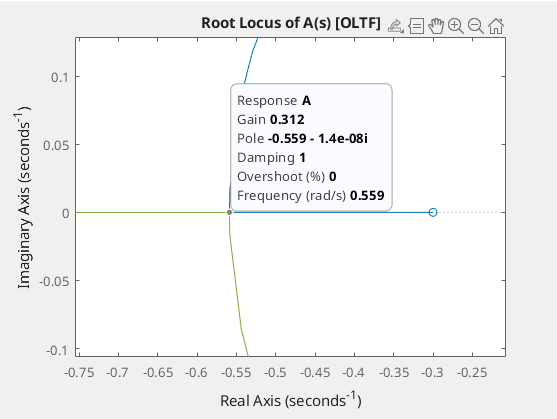
\includegraphics[width=0.8\textwidth]{figures/root_locus_s3.png}
        \caption{Σημείο Σύγκλισης $s_3$}
        \label{fig:root_locus_s3}
    \end{figure}
\end{itemize}

\section{Επιλογή Ασαφούς Ελεγκτή}
Η γενικότερη δομή ενός ασαφούς PI ελεγκτή είναι η εξής:
\begin{figure}[H]
    \centering
    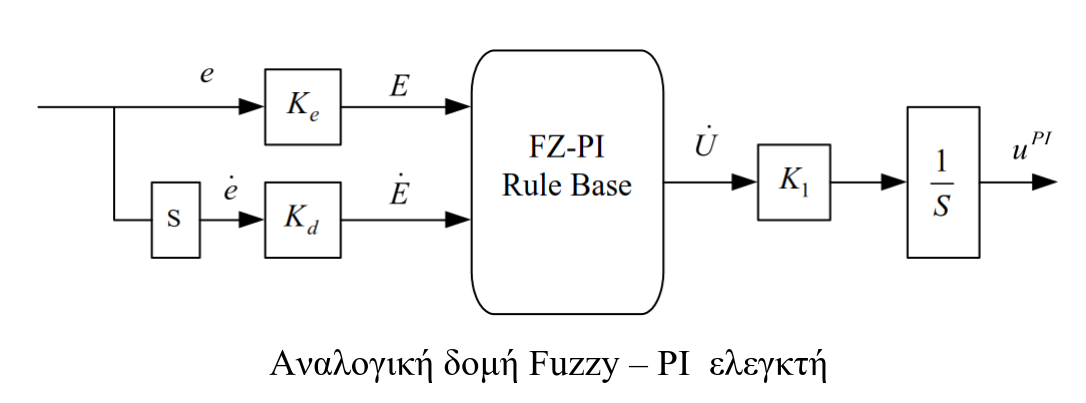
\includegraphics[width=1\textwidth]{figures/fuzzy_pi.png}
    \caption{Δομή Ασαφούς Ελεγκτή PI}
    \label{fig:fuzzy_pi_controller}
\end{figure}

Ένας ασαφής ελεγκτής FZ-PI (Fuzzy PI Controller) προσδιορίζεται από ασαφείς κανόνες της μορφής:
\begin{equation}
    \label{eq:fuzzy_rule}
    \text{IF } e(k) \text{ IS } A \text{ AND } \Delta e(k) \text{ IS } B \text{ THEN } \Delta u(k) \text{ IS } C
\end{equation}
,όπου τα A, B και C οι λεκτικές τιμές που αποδίδονται στα σφάλματα $e(k)$, $\Delta e(k)$ και $\Delta u(k)$ αντίστοιχα.

Στην προκειμένη περίπτωση οι λεκτικές τιμές των δύο εισόδων και της εξόδου παρουσιάζουν ίδιες συναρτήσεις συμμετοχής, όπως φαίνεται στο παρακάτω σχήμα:
\begin{figure}[H]
    \centering
    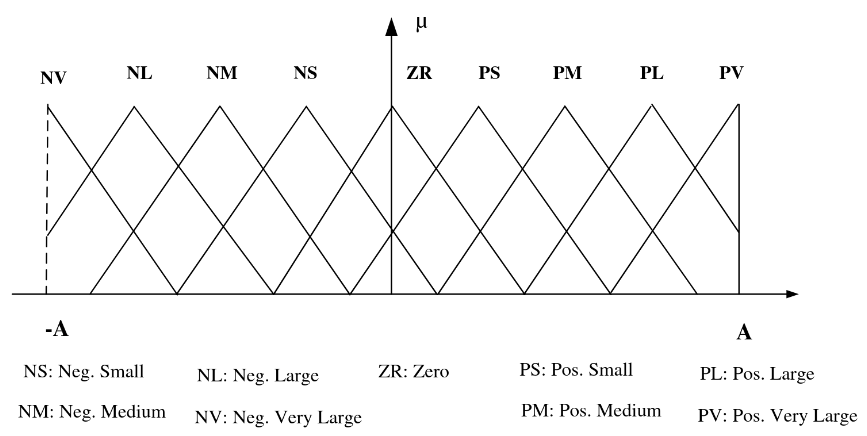
\includegraphics[width=0.8\textwidth]{figures/fuzzy_rules.png}
    \caption{Λεκτικές Τιμές Εισόδων και Εξόδου Ασαφούς Ελεγκτή}
    \label{fig:fuzzy_rules}
\end{figure}

Η γενική μορφή του ελεγκτή FZ-PI είναι παρόμοια με αυτή του ελεγκτή PI:
\begin{equation}
    \label{eq:fuzzy_pi_controller}
    \Delta u(k) = F{e(k), \Delta e(k)}
\end{equation}
\begin{equation}
    \label{eq:pi_controller}
    \Delta u(k) = K_P \cdot \Delta e(k) + K_I \cdot e(k)
\end{equation}

\begin{table}[t]
    \centering
    \begin{tabular}{|c|c|c|c|c|}
    \hline
    {$K_1$} & {$K_e$} & {$K_d$} & {Overshoot (\%)} & {Rise Time (s)} \\
    \hline
    50      & 0.0010  & 0.0002  &  2.41            & 0.4100 \\
    50      & 0.0025  & 0.0003  &  0.14            & 0.4400 \\
    50      & 0.0030  & 0.0003  &  0.27            & 0.4400 \\
    50      & 0.0035  & 0.0003  &  0.72            & 0.4600 \\
    50      & 0.0040  & 0.0003  &  3.57            & 0.4900 \\
    60      & 0.0010  & 0.0002  & -0.22            & 0.3800 \\
    60      & 0.0030  & 0.0003  &  0.21            & 0.4900 \\
    60      & 0.0035  & 0.0003  & -0.02            & 0.4800 \\
    60      & 0.0040  & 0.0003  &  0.93            & 0.4900 \\
    60      & 0.0045  & 0.0003  &  3.46            & 0.5000 \\
    70      & 0.0010  & 0.0002  & -0.19            & 0.3600 \\
    70      & 0.0035  & 0.0003  &  0.08            & 0.5300 \\
    70      & 0.0040  & 0.0003  &  0.63            & 0.5100 \\
    70      & 0.0045  & 0.0003  &  2.08            & 0.5000 \\
    70      & 0.0050  & 0.0003  &  3.95            & 0.4900 \\
    80      & 0.0010  & 0.0002  & -0.17            & 0.3400 \\
    80      & 0.0015  & 0.0002  &  4.52            & 0.2600 \\
    80      & 0.0035  & 0.0003  &  0.32            & 0.5600 \\
    80      & 0.0040  & 0.0003  &  0.70            & 0.5100 \\
    80      & 0.0045  & 0.0003  &  1.80            & 0.5000 \\
    80      & 0.0050  & 0.0003  &  3.28            & 0.4900 \\
    90      & 0.0010  & 0.0002  & -0.16            & 0.3400 \\
    90      & 0.0015  & 0.0002  &  2.44            & 0.2500 \\
    90      & 0.0035  & 0.0003  &  0.55            & 0.5700 \\
    90      & 0.0040  & 0.0003  &  0.94            & 0.5300 \\
    90      & 0.0045  & 0.0003  &  1.97            & 0.5000 \\
    90      & 0.0050  & 0.0003  &  3.23            & 0.4900 \\
    100     & 0.0015  & 0.0002  &  0.95            & 0.2300 \\
    100     & 0.0035  & 0.0003  &  0.77            & 0.5600 \\
    100     & 0.0040  & 0.0003  &  1.24            & 0.5200 \\
    100     & 0.0045  & 0.0003  &  2.26            & 0.4900 \\
    100     & 0.0050  & 0.0003  &  3.57            & 0.4800 \\
    \hline
    \end{tabular}
    \caption{Gains, Overshoot, and Rise Time for Fuzzy PI Controller}
    \label{tab:gains}
\end{table}

\begin{table}[t]
    \centering
    \begin{tabular}{|c|c|c|c|c|}
    \hline
    {$K_1$} & {$K_e$} & {$K_d$} & {Overshoot (\%)} & {Rise Time (s)} \\
    \hline
    110     & 0.0015  & 0.0002  &  0.85            & 0.2300 \\
    110     & 0.0030  & 0.0003  &  0.54            & 0.5900 \\
    110     & 0.0035  & 0.0003  &  0.98            & 0.5500 \\
    110     & 0.0040  & 0.0003  &  1.55            & 0.5200 \\
    110     & 0.0045  & 0.0003  &  2.61            & 0.4900 \\
    110     & 0.0050  & 0.0003  &  3.98            & 0.4800 \\
    120     & 0.0015  & 0.0002  &  0.68            & 0.2100 \\
    120     & 0.0030  & 0.0003  &  0.61            & 0.5700 \\
    120     & 0.0035  & 0.0003  &  1.19            & 0.5400 \\
    120     & 0.0040  & 0.0003  &  1.89            & 0.5100 \\
    120     & 0.0045  & 0.0003  &  3.00            & 0.4800 \\
    120     & 0.0050  & 0.0003  &  4.43            & 0.4700 \\
    130     & 0.0015  & 0.0002  &  0.46            & 0.2000 \\
    130     & 0.0020  & 0.0002  &  4.72            & 0.1800 \\
    130     & 0.0025  & 0.0003  &  0.04            & 0.5900 \\
    130     & 0.0030  & 0.0003  &  0.66            & 0.5500 \\
    130     & 0.0035  & 0.0003  &  1.41            & 0.5200 \\
    130     & 0.0040  & 0.0003  &  2.22            & 0.4900 \\
    130     & 0.0045  & 0.0003  &  3.39            & 0.4700 \\
    130     & 0.0050  & 0.0003  &  4.91            & 0.4600 \\
    140     & 0.0015  & 0.0002  &  0.23            & 0.1900 \\
    140     & 0.0020  & 0.0002  &  4.91            & 0.1700 \\
    140     & 0.0025  & 0.0003  &  0.07            & 0.5700 \\
    140     & 0.0030  & 0.0003  &  0.71            & 0.5300 \\
    140     & 0.0035  & 0.0003  &  1.61            & 0.5000 \\
    140     & 0.0040  & 0.0003  &  2.54            & 0.4800 \\
    140     & 0.0045  & 0.0003  &  3.77            & 0.4600 \\
    150     & 0.0015  & 0.0002  &  0.22            & 0.1900 \\
    150     & 0.0025  & 0.0003  &  0.11            & 0.5600 \\
    150     & 0.0030  & 0.0003  &  0.85            & 0.5300 \\
    150     & 0.0035  & 0.0003  &  1.78            & 0.5000 \\
    150     & 0.0040  & 0.0003  &  2.84            & 0.4800 \\
    150     & 0.0045  & 0.0003  &  4.15            & 0.4600 \\
    \hline
    \end{tabular}
    \caption{Gains, Overshoot, and Rise Time for Fuzzy PI Controller}
    \label{tab:gains2}
\end{table}


\end{document}